\documentclass{beamer}
\usepackage[utf8]{inputenc}
\usepackage[english,russian]{babel}
\usetheme{Rochester}
\usepackage{graphicx}
\usepackage{caption}
\setbeamertemplate{caption}[numbered]
%:\captionsetup[figure]{labelformat=empty}

% Настройка метаинформации
\title[Краткое название]{Расчёт режимов работы светофорных объектов}
%\subtitle{Подзаголовок презентации}
\author{Павел Попов}
\institute{
	Санкт-Петербургский политехнический университет Петра Великого\\
	\medskip
	$ $ Высшая школа прикладной математики и вычислительной физики
	}
\date{\today}


\begin{document}
	% Титульный слайд
	\begin{frame}
		\titlepage
	\end{frame}
	
	\begin{frame}{Актуальность}
		
		\begin{columns}[T]
			\begin{column}{0.6\textwidth}
				\begin{itemize}
					\item Светофорные объекты (СО) - это ключевой элемент дорожной инфраструктуры.
					\item СО организовывают движение транспорта в соответствии с определенными правилами и приоритетами.
					\item Оптимально настроенные режимы работы СО предотвращают появление заторов, улучшают пропускную способность дорожного участка, который регулируют.
				\end{itemize}
			\end{column}
			\begin{column}{0.4\textwidth}
				\begin{figure}
					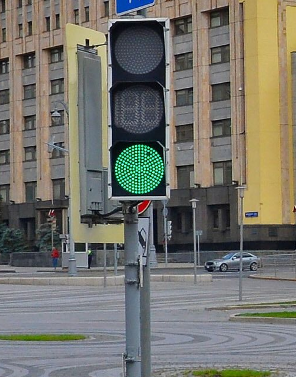
\includegraphics[width=\textwidth]{images/tr-l.png}
					Светофорный объект
					\label{fig:traffic_light}
				\end{figure}
			\end{column}
		\end{columns}
	\end{frame}
	
	\begin{frame}{Актуальность}
		\begin{itemize}
			\item Настройка длительностей действия регулирующих сигналов в реальном времени не представляется возможной, т.к. может создать аварийную ситуацию на дорожном участке.
		\end{itemize}
		Для решения этой проблемы применяется подход \textit{микромоделирование} автомобильного трафика.
		\begin{itemize}
			\item На основании статистических данных строится правдоподобная модель ситуации на дороге.
		\end{itemize}
		Микромоделирование предоставляет возможности:
		\begin{itemize}
			\item Проводить виртуальные эксперименты.
			\item Анализировать воздействие сигналов СО на поток транспорта. 
		\end{itemize}
	\end{frame}
	
	\begin{frame}{Постановка задачи}
		\begin{itemize}
			\item Предстоит решить проблему расчётов режимов работы СО при помощи технологии микромоделирования автомобильного трафика на дорожном участке.
			\item Представим проблему в виде целочисленной задачи оптимизации с ограничениями.
		\end{itemize}
		
		\begin{block}{Задание дорожного участка}
			Участок транспортной сети опишем в виде ориентированного графа $\Gamma(V,E)$, где $V$ - множество вершин, $E$ - множество дуг сети.\\
		\end{block}
		
	\end{frame}
	
	\begin{frame}{Постановка задачи}
		Из $V$ выделим подможества $S\subseteq V$, $D\subseteq V$ и дадим опр-я:
		\begin{block}{Определение}
			\textit{Источником} называется элемент множества $S$, который порождает транспортный поток.
		\end{block}
		\begin{block}{Определение}
			\textit{Стоком} называется элемент множества $D$, который поглощает транспортный поток.
		\end{block}
		\begin{itemize}
			\item Каждая дуга соответствует реальному участку автодороги без перекрёстков
			(дорожной полосе).
			\item Каждая вершина представляет собой либо перекрёсток, регу­лируемый светофорным объектом, либо является источником, либо стоком либо
			источником и стоком одновременно.
		\end{itemize}
		 
	\end{frame}
	
	\begin{frame}{Постановка задачи}
		\begin{block}{Определение}
			Множество $W$ всех потокообразующих пар представим в виде декартова произведения 
			\begin{equation}
				W = S \times D = \{\omega = (i, j): \ i \in S, j \in D\}
			\end{equation}
		\end{block}
		\begin{block}{Определение}
			Путём (маршрутом) в сети $\Gamma$, соединяющим вершины $i$ и $j$, назовём последовательность дуг
			\begin{equation}
				\scriptstyle e_1 = (i\rightarrow k_1), \ e_2 = (k_1 \rightarrow k_2), \ \ldots, \ e_m = (k_{m-1} \rightarrow k_m), \  e_{m+1} = (k_m \rightarrow j)
			\end{equation}
			где $e_l \in E$ при всех $l = 1,\ldots, m+1$
		\end{block}
	\end{frame}
	
	\begin{frame}{Постановка задачи}
		\begin{itemize}
			\item Обозначим через $P_w$ множество альтернативных маршрутов, связывающих пару $w \in W$.
			\item Совокупность всех путей в сети $\Gamma$ обозначим через $P = \underset{\omega \in W}{\cup}P_{\omega}$.
			\item В маршрутах предполагается отсутствие петель и циклов.
			\item Автомобили перемещаются по маршрутам из $P$.
			\item Пользователями дорожной сети будем считать только автомобили.
		\end{itemize}
	\end{frame}
	
	\begin{frame}{Постановка задачи}
		\begin{itemize}
			\item Выделим из множества $V$ подмножество $O \subset V$, $|O| = N, N \in \mathbb{N}$ вершин - светофорных объектов.
			\item $o_i\in O, \ i = 1,\ldots, N$ регулируют состояние потока автомобилей на инцидентных $o_i$ дугах, входящих в $o_i$, с помощью сигналов.
			\item Введём три вида сигналов: красный, жёлтый, зелёный.
			\item Объединим сигналы в мн-во $$\mathcal{L} = \{ l_d \}, \ d = 1, \ldots, M, \ M \in \mathbb{N}.$$
		\end{itemize}	
	\end{frame}
	
	\begin{frame}{Постановка задачи}
		\begin{block}{Фаза СО}
			\textit{Фаза} $p_{lk}$- это $k$-ое, $ k = 0, \ldots, K, k \in \mathbb{N}$ \textit{состояние} $l$-го СО, поддерживаемое в течение времени $t_{lk}$, $t_{lk} \in \mathbb{N}$, \ $t_{\min} \leq t_{lk} \leq t_{\max}$, \ $[t_{lk}] = \text{с}$.
		\end{block}
		\begin{block}{Состояние СО}
			Под \textit{состоянием} понимается совокупность влияний сигнала $l_d$ на инцидентные входящие в $l$-ый СО дуги $e_j$ в фазе $p_{lk}$.\\
		\end{block}
	\end{frame}
	
	\begin{frame}{Постановка задачи}
		Пусть:
		\begin{itemize}
			\item $X = \biggr[t_{lk}\biggl]_{\begin{aligned}
					\scriptstyle l & \scriptstyle \in 1,\ldots, N,\\
					\scriptstyle k & \scriptstyle \in 0, \ldots, K
			\end{aligned}}, X \in \mathbb{R}^{N\cdot K}$ вектор, содержащий длительности фаз светофорных объектов.
			\item $T[\text{с}]$ - продолжительность времени симуляции трафика.
			\item $\mathcal{N}$ - количество ТС, преодолевших полные намеченные пути (маршруты) за время $T$.
			\item \textit{Время ожидания} (\textit{простоя}) $\tau_i(X)$ $i$-ого ТС - время, в течение которого скорость $v$ ТС удовлетворяет ограничению $v < 0.1 \ \frac{\text{м}}{\text{c}}$.\\
		\end{itemize}
	\end{frame}
	
	\begin{frame}{Постановка задачи}
		\begin{block}{Функция цели}
			Пусть $\tau_i$ - время ожидания $i$-ой машины. Тогда
			\begin{equation}
				\displaystyle f(X) = \frac{\sum\limits_{i = 1}^{\mathcal{N}}\tau_i}{\mathcal{N}}
			\end{equation} - функция цели.\\
		\end{block}
		\begin{block}{Задача оптимизации}
			\begin{equation}
				\label{eq:goal-function}
				\begin{aligned}
					\min \quad & f(X) \\
					\text{s.t.} \quad & t_{lk} \in [t_{\min}, t_{\max}]\
				\end{aligned}	
			\end{equation}
		\end{block}
	\end{frame}
	
	\begin{frame}{Анализ существующих решений}
		Tunc I., Soylemez M. Fuzzy logic and deep Q learning based control for traffic lights // Alexandria Engineering Journal. — 2023. — Т. 67. — С. 343—359.
		\begin{itemize}
			\item Каждый перекрёсток регулируется СО.
			\item Алгоритмы ML отвечают за смену последовательностей фаз СО.
			\item Изменение длительности зелёного сигнала СО контролируют алгоритмы, основанные на нечеткой логике.
			\item Данные о трафике контролируются при помощи камер видеонаблюдения.
		\end{itemize}
	\end{frame}
	
	\begin{frame}{Анализ существующих решений}
		Samra S., El-Mahdy A., Wada Y. A Linear Time and Space Algorithm for
		Optimal Traffic-Signal Duration at an Intersection // IEEE Transactions on Intelligent
		Transportation Systems. — 2015. — Т. 16, No 1. — С. 387—395.
		\begin{itemize}
			\item Подход, основанный на динамическом программировании.
			\item Миркромоделирование не производится.
			\item На основании исторических данных предлагается предсказывать, какое количество ТС пересечёт перекресток в течение каждой из фаз в будущем.
			\item Предсказанные значения трафика используются в последующих шагах алгоритма.
		\end{itemize}
	\end{frame}
	
	\begin{frame}{Анализ существующих решений}
		Solving Traffic Signal Setting Problem Using Machine Learning / P. Gora
		[и др.] // 2019 6th International Conference on Models and Technologies for Intelligent
		Transportation Systems
		\begin{itemize}
			\item Использование суррогатной модели для вычисления значения ЦФ.
			\item Оптимизация длительностей фаз при помощи метаэвристических алгоритмов оптимизации.
			\item Сбор данных о трафике при помощи спутников и использование Floating Car Data.
		\end{itemize}
	\end{frame}
	
	\begin{frame}{Анализ существующих решений}
		Sun D., Benekohal R. ( F., Waller S. T. Bi-level Programming Formulation
		and Heuristic Solution Approach for Dynamic Traffic Signal Optimization // Computer–Aided Civil and Infrastructure Engineering. — 2006. — Т. 21.
		\begin{itemize}
			\item Представление проблемы в виде двухуровневой задачи оптимизации.
			\item Задача верхнего уровня - расстановка длительностей действия сигналов СО.
			\item Задача нижнего уровня - распределение маршрутов ТС.
			\item Данные о трафике - матрица корреспонденций.
		\end{itemize}
	\end{frame}
	
	\begin{frame}{Анализ существующих решений}
		Chen S., Yang C.-B., Peng Y.-H. Algorithms for the Traffic Light Setting
		Problem on the Graph Model. — 2007.\\
		Zine-dine K., Madani A. USING PSO ALGORITHM FOR THE TRAFFIC
		LIGHTS SETTING PROBLEM WITH CELLULAR AUTOMATON MODEL 1 //. —
		2013.
		\begin{itemize}
			\item Дорожная сеть задаётся в виде ориентированного графа.
			\item Используются дискретные модели или модели на основе дискретных.
			\item Данные о трафике - матрица корреспонденций.
			\item Имеют место значительные допущения в постановке задач.
		\end{itemize}
	\end{frame}
	
	\begin{frame}{Предлагаемый алгоритм}
		Предлагается решить задачу оптимизации (\ref{eq:goal-function}) при помощи метаэвристических алгоритмов:
		\begin{itemize}
			\item Генетический алгоритм;
			\item Метод роя частиц;
			\item Эволюционная стратегия с адаптацией матрицы ковариаций (CMA-ES).
		\end{itemize}
		При помощи фреймворка SUMO:
		\begin{itemize}
			\item Задать дорожную сеть, светофорные объекты, состояния, фазы.
			\item Задать движение потока ТС, моделью\\ Intelligent Driver Model (IDM).
			\item Обеспечить вычисление значения ЦФ.
		\end{itemize}
	\end{frame}
	
	\begin{frame}{Данные о трафике}
		\textbf{Volume} - интенсивность движения за 5 мин \bigg[$\frac{\text{ед}}{\text{5 мин}}$\bigg].
		\begin{figure}
			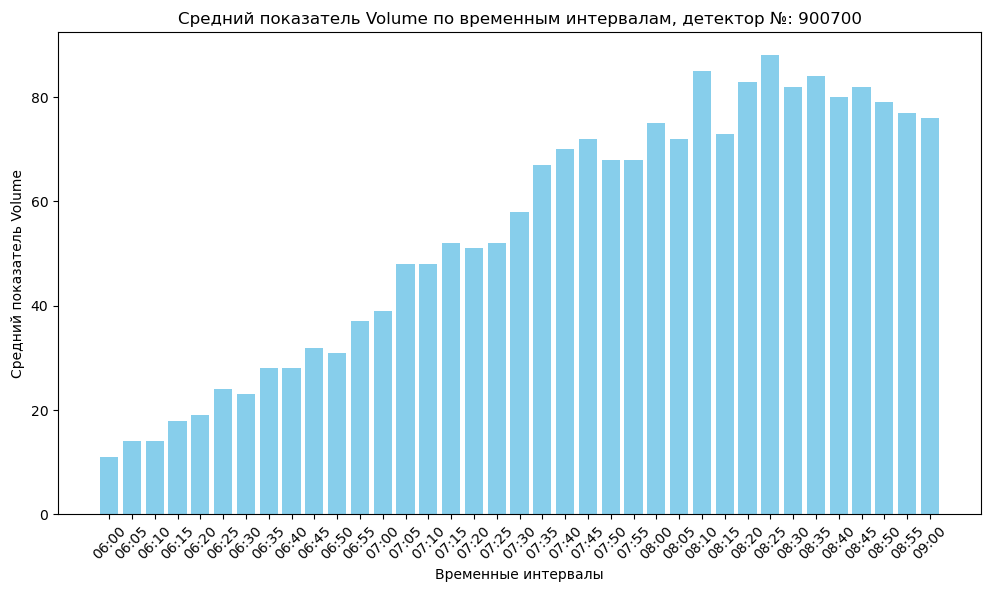
\includegraphics[width=\textwidth]{images/900700-hist-wd-avgvol.png}
			\label{traffic:hist-vol}
		\end{figure}
	\end{frame}
	
	\begin{frame}{Данные о трафике}
		\begin{figure}
			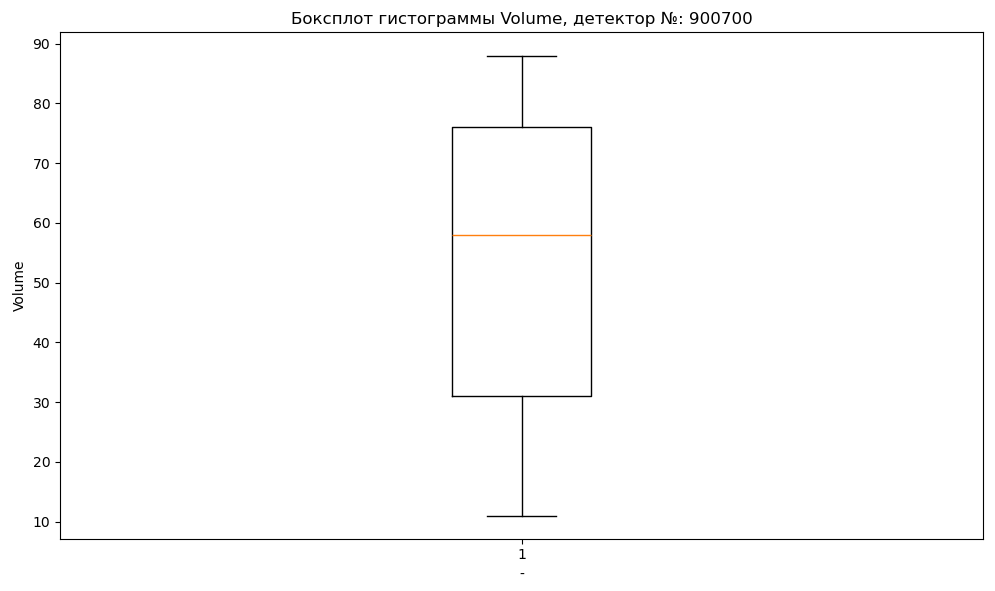
\includegraphics[width=\textwidth]{images/900700-boxplot-wd-avgvol.png}
			\label{traffic:boxplot-vol}
		\end{figure}
	\end{frame}
	
	\begin{frame}{Данные о трафике}
		\begin{figure}
			
\includegraphics[width=\textwidth]{images/900700-line-1-time-boxplots-wd-avgvol.png}
			\label{traffic:time-boxplots-vol}
		\end{figure}
	\end{frame}
	\begin{frame}{Данные о трафике}
		\textbf{Speed} - средняя скорость транспортных средств за 5 мин \bigg[$\frac{\text{км}}{\text{ч}}$\bigg].
		\begin{figure}
			
\includegraphics[width=\textwidth]{images/900700-line-1-time-boxplots-avgspeed-wd.png}
		\end{figure}
	\end{frame}
	
	\begin{frame}{Данные о трафике}
		\begin{figure}
			
\includegraphics[width=\textwidth]{images/wd-vol-boxplots.png}
		\end{figure}
	\end{frame}
	
	\begin{frame}{Данные о трафике}
		\begin{figure}
			
\includegraphics[width=\textwidth]{images/wd-speed-boxplots.png}
		\end{figure}
	\end{frame}
	
	\begin{frame}{Дорожный участок}
		\begin{figure}
			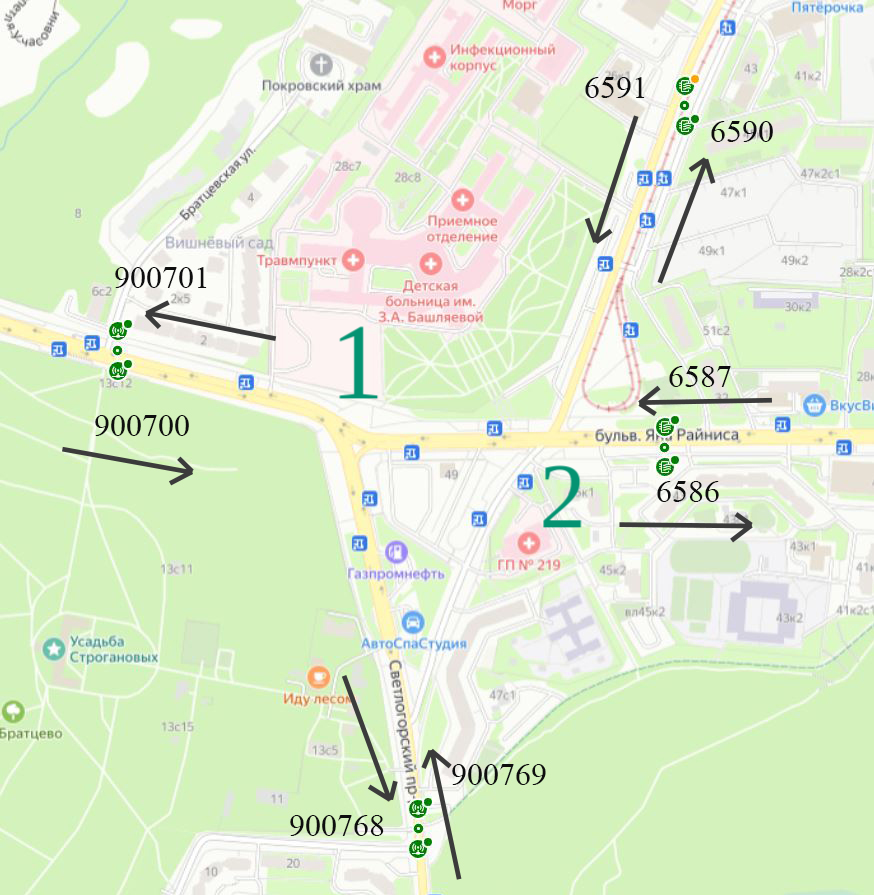
\includegraphics[width=0.65\textwidth]{images/radiodetectors.png}
		\end{figure}
	\end{frame}
	
	\begin{frame}{Места установки детекторов}
		\begin{figure}
			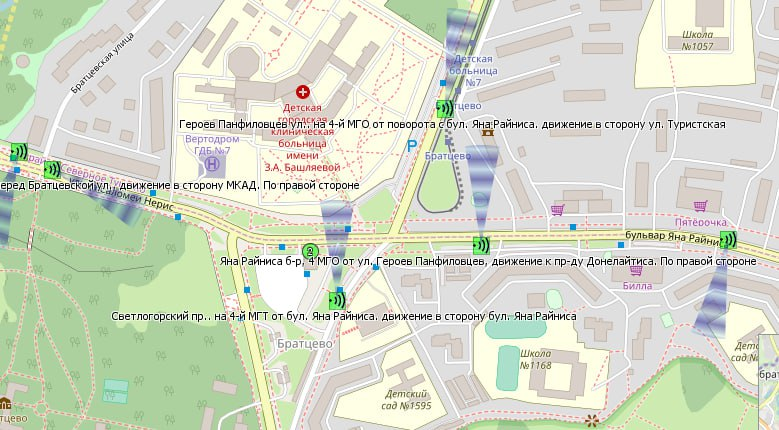
\includegraphics[width=\textwidth]{images/detectors-mapping.jpg}
		\end{figure}
	\end{frame}
	
	\begin{frame}{Модель дорожного участка, пример состояния}
		\begin{figure}
			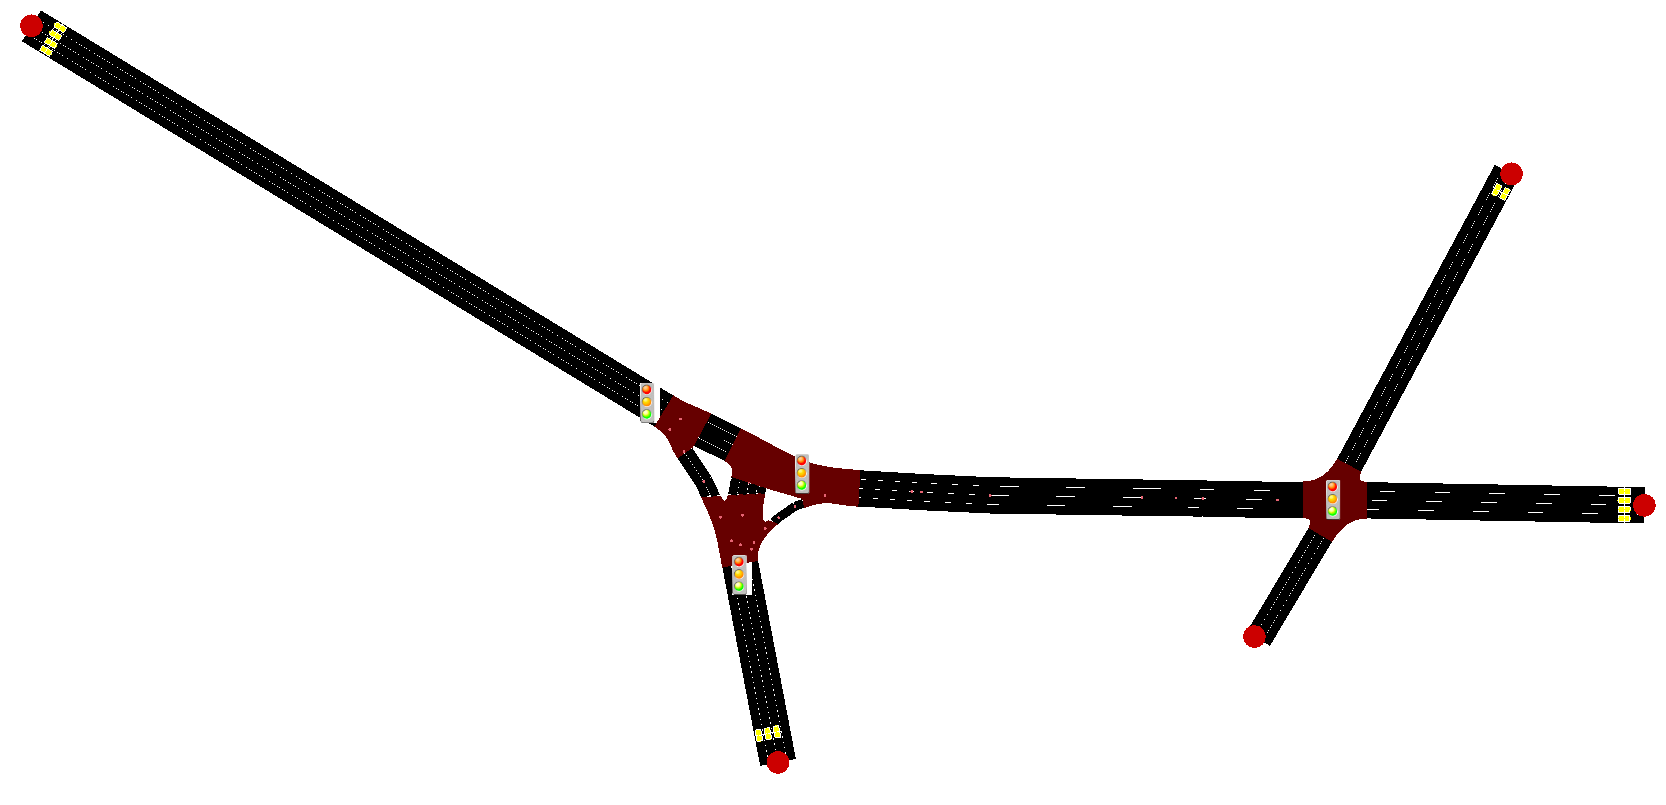
\includegraphics[width=0.8\textwidth]{images/detectors-setting.png}
		\end{figure}
		\begin{figure}
			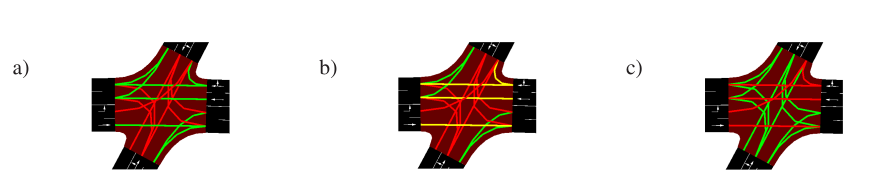
\includegraphics[width=\textwidth]{images/state-ch.png}
			\label{map:detectors-mapping}
		\end{figure}
	\end{frame}
	
	\begin{frame}{}
		
	\end{frame}
	
\end{document}